\ylDisplay{Hooratas} % Ülesande nimi
{Valter Kiisk} % Autor
{lõppvoor} % Voor
{2007} % Aasta
{G 4} % Ülesande nr.
{5} % Raskustase
{
% Teema: Dünaamika
\ifStatement
Hooratas raadiusega $R$ pöörleb nurkkiirusega $\omega$. Lihtsuse huvides võib hooratast vaadelda peenikese rõngana (pöörlemistelg ühtib rõnga teljega).\\
\osa Milline on energia salvestustihedus $w$ (kineetiline energia massiühiku kohta) hoorattas?\\
\osa Hooratas on valmistatud süsinikkiuga armeeritud polümeerist, mille tõmbetugevus $\sigma\idx{max} = \SI{2,4e9}{Pa}$ ja tihedus $\rho = \SI{1500}{kg/m^3}$. Hinnake energia salvestustiheduse maksimaalselt võimalikku väärtust sellises hoorattas (andes numbrilise vastuse).

\emph{Vihje}. Tõmbetugevus on maksimaalne jõud ristlõike pindala kohta, mida antud materjal talub ilma purunemata.
\fi


\ifHint
Mehaaniline pinge rõngas on määratud tsentrifugaaljõu poolt, millega rõngast radiaalselt väljapoole tiritakse. Pinge täpseks määramiseks on mugav vaadelda väikest rõnga juppi ning sellele mõjuvate jõudude tasakaalu.
\fi


\ifSolution
\osa Hooratta kineetiline energia on $K = \frac{1}{2}M\omega^2R^2$, seega energia salvestustihedus $w = E/M = \frac{1}{2} \omega^2R^2$.

\osa Olgu rõnga raadius $r$ ja mass $m$. Mehaaniline pinge rõngas ($\sigma$) on määratud tsentrifugaaljõuga, millega kahte rõnga poolt üksteisest eemale tõugatakse. Vaatleme ühe rõnga poole väikest lõiku pikkusega $\Delta l$. Selle mass on $\Delta m = (\Delta l/2\pi r)m$ ja sellele mõjub tsentrifugaaljõud suurusega $\Delta F = \Delta m\omega^2 r$, kus $\omega$ on pöörlemise nurkkiirus. Selle jõu projektsioon vertikaalsihile on (vt joonist)
\[
\Delta F_{ \|}=\Delta F \cos \alpha=\frac{m \omega^{2}}{2 \pi} \Delta l \cos \alpha.
\]
Ent $\Delta l \cos \alpha$ on lõigu $\Delta l$ projektsioon horisontaalsihile. Järelikult summaarne jõud, mis mõjub ühele rõnga poolele, avaldub kui
\[
F=\sum \Delta F_{ \|}=\frac{m \omega^{2}}{2 \pi} 2 r=\frac{m \omega^{2} r}{\pi}.
\]
Teiselt poolt, $F = 2\sigma S$, kus $S$ on rõnga ristlõige. Viimase asendame seosest
\[
m=\rho V=\rho(2 \pi r S) \Rightarrow S=\frac{m}{2 \pi r \rho}.
\]
Kokkuvõttes saame
\[
\sigma = \frac{F}{2S} = \omega^2 r^2 \rho.
\]
Rõnga kineetiline energia
\[
E = \frac{mv^2}{2} = \frac{m\omega^2r^2}{2} = \frac{m\sigma}{2\rho},
\]
millest $E/m = \sigma /2\rho$. Võttes $\sigma = \sigma\idx{max}$, saame $E/m = \SI{800}{kJ/kg}$.

\begin{center}
	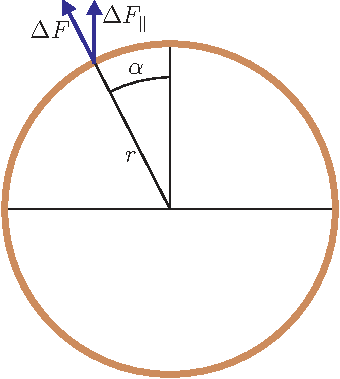
\includegraphics[width=0.45\textwidth]{2007-v3g-04-yl}
\end{center}
\fi
}